\newcommand{\functionListing}[2]{\hypertarget{#1}{\textbf{/#1/} #2}}
\newcommand{\refFnListing}[2]{\hyperlink{#1}{#2}}

\newcommand{\inputDefault}[2]{\input{../default/#1/#2}}
\newcommand{\inputDefaultByFormat}[1]{\input{../default/\documentFormat/#1}}

\newcommand{\setDocumentName}[1]{\def \documentName {#1}}
\newcommand{\setDocumentFormat}[1]{\def \documentFormat {#1}}

\newcommand{\printTitle}{\inputDefault{\documentFormat}{title}}
\newcommand{\printTableOfContents}{\tableofcontents}

\newcommand{\printListOfFigures}{\listoffigures}
\newcommand{\printBibliography}{\bibliography{../default/sources}}{\bibliographystyle{plain}}
\newcommand{\printGlossary}{\printglossary[nonumberlist]}

% Better tables
\newcommand{\HRule}{\rule{\linewidth}{0.5mm}}
\newcommand\addrow[2]{#1 &#2\\ }
\newcommand\addheading[2]{#1 &#2\\ \hline}
\newcommand\tabularhead{\begin{tabular}{lp{13cm}}\hline}
\newcommand\addmulrow[2]{ \begin{minipage}[t][][t]{2.5cm}#1\end{minipage}% 
	&\begin{minipage}[t][][t]{8cm}
	\begin{enumerate} #2   \end{enumerate}
	\end{minipage}\\ }
\newenvironment{usecase}{\tabularhead}{\hline\end{tabular}}

\newcommand{\graphic}[3]{
	\begin{figure}[H]
		\begin{center}
			\input{graphics/#1}
			\caption{#2}
			\label{#3}
		\end{center}	
	\end{figure}	
}
\setDocumentName{ERP-Evaluierung}
\setDocumentFormat{pdf}
\inputDefaultByFormat{layout}

\usepackage{hyperref}
\usepackage{amsmath}
\usepackage{amssymb}
\usepackage{booktabs}
\usepackage[pdftex]{graphicx}
\usepackage{hyperref}
\usepackage{ngerman}
\usepackage[utf8]{inputenc}
\usepackage{tabularx}
\usepackage[toc]{glossaries}
\usepackage{float}
\usepackage{multirow}
\usepackage{blindtext}
\usepackage{lipsum}
\usepackage{xargs}
\usepackage[pdftex,dvipsnames]{xcolor}
\usepackage[colorinlistoftodos,prependcaption,textsize=tiny]{todonotes}
\usepackage{xcolor}
\usepackage{listings}
\usepackage{picins}
\usepackage[autostyle]{csquotes} 

\definecolor{backcolour}{rgb}{0.95,0.95,0.92}

\lstset{ 
    basicstyle=\footnotesize\ttfamily,
    keywordstyle=\bfseries\color{BurntOrange},
	commentstyle=\itshape\color{gray},
    numbers=left, % where to put the line-numbers
    numberstyle=\tiny, % the size of the fonts that are used for the line-numbers     
    backgroundcolor=\color{backcolour},
    showspaces=false, % show spaces adding particular underscores
    showstringspaces=false, % underline spaces within strings
    showtabs=false, % show tabs within strings adding particular underscores
    frame=single, % adds a frame around the code
    tabsize=2, % sets default tabsize to 2 spaces
    rulesepcolor=\color{gray},
    rulecolor=\color{black},
    captionpos=b, % sets the caption-position to bottom
    breaklines=true, % sets automatic line breaking
    breakatwhitespace=false,
	identifierstyle=\color{blue},
	stringstyle=\color{OliveGreen},
	xleftmargin=5.0ex
}


\usepackage{tikz}
\usetikzlibrary{matrix,chains,positioning,decorations.pathreplacing,arrows}

\makeglossaries
\loadglsentries[main]{../default/glossar}

% http://tex.stackexchange.com/questions/9796/how-to-add-todo-notes
\newcommandx{\unsure}[2][1=]{\todo[linecolor=red,backgroundcolor=red!25,bordercolor=red,#1]{#2}}
\newcommandx{\change}[2][1=]{\todo[linecolor=blue,backgroundcolor=blue!25,bordercolor=blue,#1]{#2}}
\newcommandx{\info}[2][1=]{\todo[linecolor=OliveGreen,backgroundcolor=OliveGreen!25,bordercolor=OliveGreen,#1]{#2}}
\newcommandx{\improvement}[2][1=]{\todo[linecolor=Plum,backgroundcolor=Plum!25,bordercolor=Plum,#1]{#2}}
\newcommandx{\thiswillnotshow}[2][1=]{\todo[disable,#1]{#2}}


\begin{document}
	
\printTitle
\printTableOfContents
\newpage

\section{Einführung}
\blindtext
\section{Geschichte}
Josef Manner I. eröffnete 1890 ein kleines Geschäft in der nähe des Stephansdoms, wo er Tafelschokolade und Feigenkaffee verkaufte. Doch da ihm die Qualität der Schokolade seiner Lieferanten nicht gut genug war, kaufte er ein Lokal eines kleinen Schokoladenerzeugers im fünften Wiener Gemeindebezirk. Daher war er ab 1. März 1890 Inhaber der ''Chocoladenfabrik Josef Manner''. \\
Zu Beginn war Josef Manner I. noch Erzeuger, Verkäufer und Werbeagent in einer Person und lieferte seine Waren oft selbst an die Kunden. Doch bereits im Gründungsjahr musste er expandieren. Bis 1897 trug er bereits die Verantwortung für über 100 Mitarbeiter und der Firmensitz wurde in die Hernalser Kulmgasse verlagert und die Firma ''Chocolade Manner'' wurde gegründet.\\
Innerhalb eines Jahrzehnts wurde die Firma zu einen der führenden Süßwarenunternehmen der österreichisch-ungarischen Monarchie. 
Die Manner-Schnitte findet sich zum ersten Mal 1898 in einem Sortimentskatalog des Hauses Manner, und zwar unter dem eher sachlichen Namen ''Neapolitaner Schnitte No. 239''. \\
Am 16. Oktober 1900 verkaufte Josef Manners damaliger Partner seinen Anteil der Firma an Johann Riedl  und legte so den Grundstein für die bis heute währende Zusammenarbeit der Familien Manner und Riedl.
Am 23. Oktober 1913 wandelte man die Firma Josef Manner \& Co. in eine Aktiengesellschaft mit dem Namen Josef Manner \& Comp AG um. Zu dieser Zeit umfasste das Unternehmen bereits 3000 Mitarbeiter und verfügte über einen Fuhrpark mit 60 Pferden und mittlerweile auch über Produktionsanlagen auf dem modernsten Stand der damaligen Zeit. \\
Während der ersten Weltkriegs konnte sich die Firma nur mit mühen über Wasser halten, da der Arbeitsmarkt der Donaumonarchie von 56 Millionen auf die gerade noch sechs Millionen Einwohner der Ersten Republik Österreich schrumpfte. Der zweite Weltkrieg brachte die Firma um ihre letzten Vorräte.\\
Am 5. Mai 1947 verstarb der Firmengründer Josef Manner I. Doch Ende der 40. Jahre wurde das Unternehmen wieder sehr schnell und vor allem International Erfolgreich. 1960 gelang der Firma der Absprung ins Technologie-Zeitalter. Die neuartige Verpackung garantierte nicht nur eine längere Haltbarkeit, sondern auch ein leichtes Öffnen der Packung. 1964 wurde erstmals seit 1914 der Rekordumsatz überschritten werden.\\
1970 erfolgte der Zusammenschluss mit dem zweitgrößten österreichischen Süßwarenunternehmen, der Firma Napoli, Ragendorfer \& Co. 1996 wurde die Firma Walde Candita in Wolkersdorf/NÖ übernommen. 2000 feierte schließlich auch die Firma Victor Schmidt \& Söhne GmbH mit den Marken „Ildefonso“ und „Victor Schmidt Austria Mozartkugeln“ ihren Einstand in der Manner-Großfamilie. \cite{josef_manner}
\section{Produktionsstandorte}
\blindtext
\section{Mitarbeiter}
\blindtext
\section{Marken \& Produkte}
\subsection{Manner}
\piccaption[Logo Manner\cite{josef_manner_marken}]{Logo Manner\cite{josef_manner_marken}}
\parpic[r]{
\includegraphics[scale=0.5]{images/logo_manner.png}}
\enquote{\enquote{Chocolade für alle – preiswert und gut}, das war die Devise von Josef Manner I. bei der Gründung der Süßwarendynastie im Jahre 1890. Dieser Grundsatz gilt auch heute für die zahlreichen Köstlichkeiten der Marke Manner.\\\\
Erfahren Sie mehr, von den im Hause Manner gerösteten Kakaobohnen bis zu köstlichen Produktneuheiten... stets dem Motto \enquote{Manner mag man eben} folgend!
}\cite{josef_manner_marken}
\picskip{0}

\subsection{Casali}
\piccaption[Logo Casali\cite{josef_manner_marken}]{Logo Casali\cite{josef_manner_marken}}
\parpic[r]{
\includegraphics[scale=0.5]{images/logo_casali.png}}
\enquote{Die Geschichte der Firma Casali reicht weit zurück in die Vergangenheit. Im Jahr 1782 gründete Joseph Casali in der damals zur k. u. k. Monarchie gehörenden Hafenstadt Triest seine Firma. Seit 1970 ist Casali, bekannt für köstliche Rum-Kokos Kugeln und fruchtige Schoko-Bananen, Teil der Josef Manner \& Comp. AG.\\\\
Wir freuen uns, Sie unter dem Motto \enquote{Welcome to Casali} auf einer virtuellen Insel voller Schoko-Früchte und exotischer Schoko-Kugeln begrüßen zu dürfen!
}\cite{josef_manner_marken}
\picskip{0}

\subsection{Victor Schmidt}
\piccaption[Logo Victor Schmidt\cite{josef_manner_marken}]{Logo Victor Schmidt\cite{josef_manner_marken}}
\parpic[r]{
\includegraphics[scale=0.5]{images/logo_victorschmidt.png}}
\enquote{Die weltberühmten Mozartkugel erweist nicht nur Wolfgang Amadeus Mozart die Ehre. Sie wurde im Laufe der Jahrzehnte ähnlich der Manner Schnitte ein Synonym für österreichische Süßwarentradition - eng verbunden mit österreichischer Hochkultur.\\\\
Lernen Sie die feinen Besonderheiten der unvergleichlichen Victor Schmidt Austria Mozartkugel kennen! LiebhaberInnen feinsten Marzipans, zarten Nougats und knackiger Bitterschokolade werden begeistert sein...}\cite{josef_manner_marken}
\picskip{0}

\subsection{Ildefonso}
\piccaption[Logo Ildefonso\cite{josef_manner_marken}]{Logo Ildefonso\cite{josef_manner_marken}}
\parpic[r]{
\includegraphics[scale=0.5]{images/logo_ildefonso.png}}
\enquote{Die Geschichte von Ildefonso ist nicht nur eine süße, sondern auch eine interessante. Sie begann gegen Ende des 19. Jahrhunderts. Im Jahr 1880 entwickelte ein Konfektmeister von Victor Schmidt die feine Rezeptur des beliebten Schicht-Nougatwürfels. Mit 1. Jänner 2000 wurde die Firma Victor Schmidt \& Söhne von Manner erworben.\\\\
Lernen Sie die vielschichtigen Seiten des beliebten Wiener Nougat-Konfekts kennen. Ein besonderes Highlight für den täglichen digitalen Genuss: jetzt auch online – die in jedem Produkt versteckten Lebensweisheiten!}\cite{josef_manner_marken}
\picskip{0}

\subsection{\#winak}
\piccaption[Logo \#winak\cite{josef_manner_marken}]{Logo \#winak\cite{josef_manner_marken}}
\parpic[r]{
\includegraphics[scale=0.5]{images/logo_winak.png}}
\enquote{Dragee Keksi von Napoli spielen eine besondere Rolle im Napoli Produktsortiment. Daher haben sie einen eigenen Online Auftritt, der diesem österreichischen Keks-Klassiker in unterhaltsamer Art und Weise gerecht wird.
Lernen Sie das Motto der Dragee Keksi \enquote{wenn ich nur aufhör`n könnt`} persönlich kennen. Unter dem Hashtag \#winak sorgen Dragee Keksi für eine nicht enden wollende Portion Spaß im digitalen Alltag!}\cite{josef_manner_marken}
\picskip{0}

\subsection{Napoli}
\piccaption[Logo Napoli\cite{josef_manner_marken}]{Logo Napoli\cite{josef_manner_marken}}
\parpic[r]{
\includegraphics[scale=0.5]{images/logo_napoli.png}}
\enquote{Unter der Marke Napoli bieten wir hochwertige Produkte für besonders preisbewußte KonsumentInnen an. Abseits der Dragee Keksi von Napoli umfasst das Sortiment vorwiegend Waffelprodukte, wie beispielsweise den Napoli Schnittenblock. Einen eigenen Online-Auftritt haben die Napoli Produkte derzeit nicht.\\\\
Bei Fragen zu Napoli Produkten abseits der Dragee Keksi bitten wir Sie, unser Kontaktformular zu verwenden. Wir danken für Ihr Verständnis.}\cite{josef_manner_marken}
\picskip{0}

\section{Qualität}
\subsection{Allgemein}
Laut Aussage von Manner, wurde die Rezeptur der Manner Original Neapolitaner Schnitte seit ihrer Erfindung durch Josef Manner I. im Jahre 1898 nicht verändert. Auch die Rezeptur anderer Produkte aus dem Manner-Sortiment ist gleich geblieben. \cite{josef_manner} \\\\
\noindent
Manner legt höchsten Wert auf ausgewählte, hochqualitative Zutaten. Bei der Anlieferung von Zutaten, werden diese in Qualitätsssicherungslabors überprüft. Vor diesem Schritt werden keine Zutaten für die Produktion freigegeben. Manner möchte mit den Lieferanten eine langjährige geschäftliche Beziehung eingehen, um eine konstant hohe Qualität sicherstellen zu können. \cite{josef_manner} \\
Auch während der laufenden Produktion wird die Qualität der Produkte überprüft. Beispielsweise werden täglich Stichproben gezogen und von einem Verkoster-Team überprüft und bewertet. \cite{josef_manner}
\subsection{International Food Standard}
Die kontinuierliche Verbesserung des Qualitätsstandard gehört zu den Grundpfeilern des Unternehmenserfolges. Daher setzt sich das Unternehmen ständig neue Ziele. Seit 2005 ist Manner nach dem besonders strengen Qualitätsstandard ''IFS'' (International Food Standard).\cite{josef_manner}\\\\
\noindent
Der IFS wurde zur Auditierung von Eigenmarkenlieferanten entwickelt. Er dient der Überprüfung der Lebensmittelsicherheit und des Qualitätsniveaus der Produzenten. Ziel dieses Standards ist es, die Lebensmittelsicherheit und Qualität der Produkte zu verbessern, den Schutz und das Vertrauen der Verbraucher zu stärken, und zusätzlich die Kosteneffizienz in der Lebensmittelkette zu erhöhen. \cite{qualityaustria_ifs}\\\\
Im Jahr 2015 hat Manner die Zertifizierung verlängern lassen und damit wieder den maximalen Standard für alle drei Manner-Produktionsstandard erreicht.
\subsection{Grundregel aus dem Manner-Verhaltenskodex}

\textit{''Unseren Marken wird viel Vertrauen und Sympathie entgegengebracht. Jeder Mitarbeiter ist verantwortlich dafür, dass unsere Produkte den Konsumenten in bestmöglicher Qualität erreichen.''} - Manner Verhaltenskodex \cite{josef_manner}
\section{Logistik}
\blindtext
\section{Konkurrenz}
\subsection{Ferrero}
Ferrero ist ein italienischer Süßwarenhersteller, welcher international, inklusive Österreich, mit 21 Produktionsstätten tätig ist. Das Unternehmen beschäftigt ca. 34.236 Mitarbeiter und erwirtschaftete 2014 einen Umsatz von 8,4 Milliarden Euro. \cite{wiki_ferrero} \\\\
Mit Produkten wie Duplo, der Milchschnitte und Nutella und dem generell breiteren Produktspektrum ist Ferrero ein durchaus ernstzunehmender Konkurrent für Manner.
\subsection{Bahlsen}
Das deutsche Familienunternehmen mit Sitz in Hannover wurde 1889 von Hermann Bahlsen gegründet. Bahlsen beschäftigt 2537 Mitarbeiter (Stand 2013) und erwirtschaftete 2013 526 Mio. Euro. \cite{wiki_bahlsen}\\\\
Bahlsen ist Marktführer in Deutschland und europaweit einer der führenden Anbieter von Süßgebäck. Das Unternehmen besitzt ebenfalls die nationalen Marken Kornland (Österreich), Krakuski (Polen) und Brandt (Deutschland). Die Produkte werden an fünf europäischen Standorten produziert und in mehr als 80 Länder exportiert. \cite{bahlsen}
\subsection{S. Spitz GmbH}
Spitz ist ein großer österreichischer Nahrungsmittelhersteller. Der Firmensitz liegt in Attnang-Puchheim, Oberösterreich. Spitz produziert hauptsächlich für den österreichischen Markt, ein Drittel der Produkte wird exportiert. Im Jahr 2005 betrug die Mitarbeiteranzahl 650 und der Umsatz 200 Mio. Euro. \cite{wiki_spitz} \\\\
Neben alkoholfreien Getränken und Spirituosen, bietet Spitz auch Backwaren, darunter auch sechs verschiedene Waffelsorten, an. \cite{spitz_produkte}
\section{Zukunftsaspekte}
Manner investiert zurzeit 40 Mio. Euro in den Ausbau des Standorts in Wien-Hernals. Dabei soll die Waffelproduktion gesteigert und die Energieverwertung effizienter werden.\\
Die aus dem Backprozess entstehende Abwärme soll ab Herbst 2016 in das lokale Fernwärmenetz eingespeist und für Heizung und Warmwasser verwendet werden. Mit der Leistung von 1 Megawatt können 600 Haushalte in unmittelbarer Nachbarschaft der Waffelproduktion profitieren. Zusätzlich wird überschüssige Abwärme des Herstellungprozesses in Kälte um und verwendet diese für Kühlzwecke.\\
Laut den Angaben von Manner können so 1.000 Tonnen CO2 pro Jahr eingespart werden. \cite{wienat_waerme}
\section{ERP-Evaluierung mittels Trovarit}
Unsere Auswahl wurde mit dem IT-Matchmaker Account vana\_gruppe\_9 durchgeführt


\subsection{Software-Kategorie}
\subsubsection{Art der gesuchten Software-Lösung}
Prozessfertigung\\
\enquote{Den meist in kleinen Stückzahl hergestellten Produkten des Maschinenbaus steht bei Pro- zessfertigern eine geringere Produktvielfalt gegenüber, die jedoch meist in groößeren Men- gen, zumindest aber mit höherer Wiederholhäufigkeit aufgelegt wird.} \cite{trovarit_prozessfertigung}

\subsection{Projektsteckbrief}
\subsubsection{Größe Ihres Unternehmens}
500-999 Mitarbeiter
\subsubsection{Anzahl Software-Arbeitsplätze für gesuchte Lösung}
60-99 Arbeitsplätze
\subsubsection{Angestrebtes Projektbudget}
bis ca. 1.000.000 EURO
\subsubsection{Angestrebte Laufzeit des Einführungsprojektes}
12-24 Monate
\subsubsection{Angestrebte Laufzeit des Einführungsprojektes}
Kurze Einführungsdauer (bis ca. 2 Monate), weil \enquote{Plug \& Play} wäre zu kurzfristig und würde zu einer Überforderung der Mitarbeiter führen
\subsubsection{Ausschlaggebende Aspekte für Ihre Investitionsentscheidung}
\begin{itemize}
	\item Funktionale Eignung der Software
	\item Günstige Betriebskosten
	\item Überlebensfähigkeit des Anbieters, da das Produkt möglichst lange genutzt werden soll
\end{itemize}
\subsubsection{Angestrebtes Preis- / Auslieferungsmodell}
Nicht relevant

\subsection{Brancheneignung}
\subsubsection{Gewünschte Branchenausrichtung der gesuchten Software}
Handel mit Lebensmitteln \& Frischeprodukten

\subsection{Unternehmenstyp}
\subsubsection{Kundenstruktur Ihres Unternehmens}
Endkundengeschäfte (B2C) und Business to Bussines to Customer (indirekter Vertrieb an Endkunden). Da die Josef Manner \& Comp. AG einerseits an Supermärkte liefert andererseits aber auch direkt an Kunden verkauft.
\subsubsection{Fertigungsart Ihres Unternehmens}
Großserien-, Massenfertigung

\subsubsection{Fertigungs-/ Produktionstyp Ihres Unternehmens}
Prozessfertigung, siehe Art der gesuchten Software-Lösung

\subsection{Software-Funktionalität}
Da diese Kriterien keine KO-Kriterien beinhalten, sondern nur für die Reihung der Systeme benötigt werden sind diese hier nicht näher beschrieben. Diese sind IT-Matchmaker unter der Vana\_Gruppe\_9 einsehbar.


\subsection{Technologie\& Sprachen}
Die folgenden Punkte wurden in Trovarit ausgewählt, andere Punkte wie Kommunikationsstandards, Software-Frameworks oder Datenformate sind für die Auswahl des Systeme irrelevant.
\subsubsection{Unterstützung folgender Clients}
PC ab Windows 7: Kritisch\\
PC Windows 10: Optional\\
Linux \& Mac: Gefordert
\subsubsection{Unterstützung folgender mobiler Clients}
Für die Auswahl des Systems Irrelevant
\subsubsection{Unterstützung folgender Sprachen}
Deutsch und Englisch: Kritisch

\subsection{Standorte des Anbieters}
\subsubsection{Support-Standorte}
Wien und generell Österreich da es ein österreichisches Unternehmen ist.
\subsection{Dienstleistung}
\subsubsection{Welche Dienstleitungen benötigen Sie zur Systemeinführung?}
\begin{enumerate}
	\item Systempräsentation mit kundenspezifischer Konfiguration: Kritische Anforderung, weil wir uns ein Bild vor der Einführung machen wollen
	\item Anpassungsprogrammierung: Optional, da ein passendes Produkt nicht weiter angepasst werden muss.
	\item Implementierung der Hardware: Kritisch, da die Hardware nicht vorhanden ist.
	\item Implementierung und Konfiguration des Netzwerkes: Kritisch, da das Netzwerkes nicht vorhanden ist.
	\item Schulung der Anwender: Kritisch, da die unerfahrenen Anwender erst geschult werden müssen.
	\item Datenmigration und Datenübernahme: Kritisch weil keine Daten verloren gehen sollen.
\end{enumerate}
\subsubsection{Welche Arten von Schulungen werden gesucht?}
Schulung im Haus des Kunden: Kritisch, um sicher zu stellen, dass alle Mitarbeiter geschult werden

\subsubsection{Welche Unterstützung benötigen Sie im Produktivbetrieb?}
\begin{enumerate}
	\item Hotline: Kritische
	\item Einsatzanalyse \& -optimierung (Audit)
\end{enumerate}

\subsubsection{Welche Dienstleistungen benötigen Sie im Bereich des Application Service Providing (ASP) / Software as a Service (SaaS)?}
Wird nicht benötigt.
\newpage
\subsection{Ergebnis}
Der Gewinner der Auswahl ist \textit{itelligence AG / itelligence ERP Branchenlösungen} mit 94\%. Mit Partnerprodukten wird sogar eine 100 \%ige Abdeckung des Funktionsumfangs erzielt. 

\begin{figure}[H]
\begin{center}
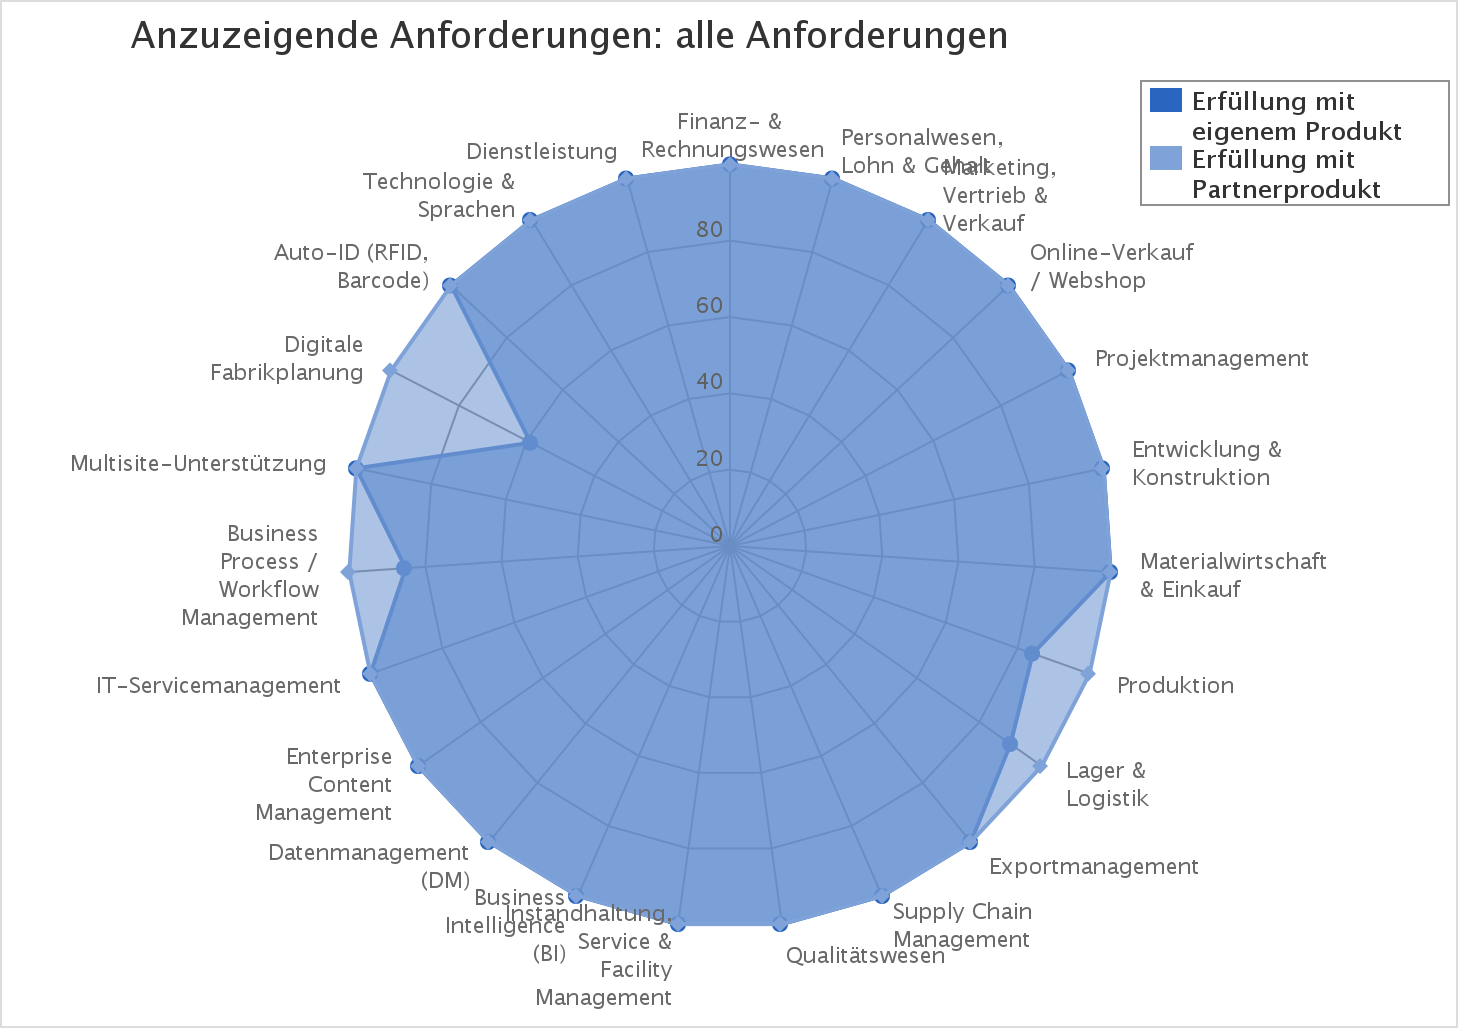
\includegraphics[width=15cm]{images/chart.png}
\caption{Spinnendiagramm}
\end{center}
\end{figure}
\noindent
Das Partnerprodukt ist vorallem für die Transport- \& Tourenplanung sowie für die Digitale Fabriksplanung (Flächenbedarfsbestimmung, Layoutgestaltung) notwendig.


\newpage
\printListOfFigures
\newpage
\printBibliography
\newpage
%\printGlossary
\end{document}